\documentclass[a4paper]{article}

\usepackage{amsmath}
\usepackage{float}
\usepackage{graphicx}
\usepackage{caption}
\usepackage{subcaption}
\usepackage{hyperref}
\usepackage[all]{hypcap}

\title{GVF Snakes}
\author{Xeryus Stokkel (s2332795)}

\begin{document}

\maketitle

\section*{Exercise 1}
The classic snake adapts to the U-shape very slowly. It often takes 300+ iterations for the circle to match the largest part of the shape as shown in \autoref{fig:firstu}. The best that I've been able to match the snake to the shape is shown in \autoref{fig:bestu}. The settings used for this are $\alpha=0.05, \beta=0, \gamma=1, \kappa=0.3, D_\text{min}=0.2, D_\text{max}=2$ and it takes 600 to 700 iterations to match this well. Changing settings during the run seems to alter the results as well, but often not for the better. Lowering $\alpha$ after every 100 iterations for example seems to improve matching to the dip since the snake gets more freedom to fit to that narrow shape, but having a very low $\alpha$ at the start means that the global shape is matched poorly because not all the dots move in unison.

The GVF snake in contrast perfectly matches the shape even with the default settings as shown in \autoref{fig:firstgvf}. This image was obtained with the default settings after just 100 iterations. So GVF snake is clearly better since it both matches the shape and it needs less time to do so.

\begin{figure}
	\centering
	\begin{subfigure}[t]{.3\textwidth}
		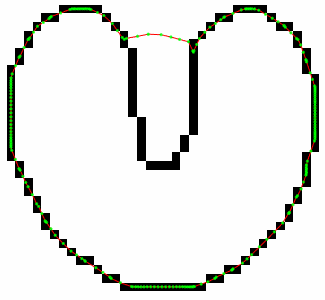
\includegraphics[width=\textwidth]{firstu}
		\caption{Classical snake with default settings and 300 iterations, this is the best attainable result with the default settings.}
		\label{fig:firstu}
	\end{subfigure}~
	\begin{subfigure}[t]{.3\textwidth}
		\centering
		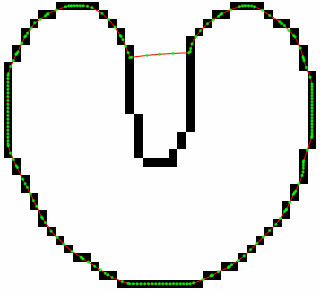
\includegraphics[width=\textwidth]{bestclassicalu}
		\caption{Best matching result that can be found with the classical snake.}
		\label{fig:bestu}
	\end{subfigure}~
	\begin{subfigure}[t]{.3\textwidth}
		\centering
		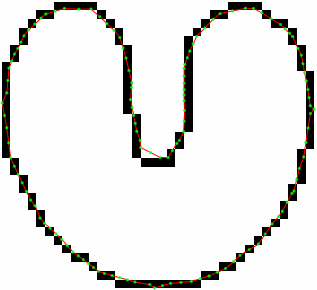
\includegraphics[width=\textwidth]{gvffirst}
		\caption{Results of using a GVF snake on the U-shape after 100 iterations.}
		\label{fig:firstgvf}
	\end{subfigure}
	\caption{Different results of matching the snake to the U-shape}
\end{figure}

\section*{Exercise 2}
The classical snake can match the room perfectly with default settings after 600 to 700 iterations. The GVF snake in contrast only needs about 10 iterations with default settings. Although it is faster GVF does not match the image as well. It appears that GVF has more trouble matching the sharp corners. Increasing both $\alpha$ and $\kappa$ makes the classical snake act more like GVF, it both matches the shape in fewer iterations (as few as 100 for $\alpha=0.5, \kappa=5$) but the sharp corners are more rounded just like GVF as well. Comparisons are shown in \autoref{fig:ex2}

\begin{figure}
	\centering
	\begin{subfigure}[t]{.3\textwidth}
		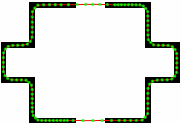
\includegraphics[width=\textwidth]{firstclass}
		\caption{Classical snake with default settings after 700 iterations}
	\end{subfigure}~
	\begin{subfigure}[t]{.3\textwidth}
		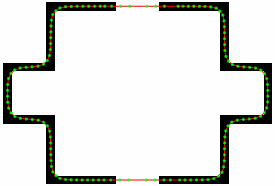
\includegraphics[width=\textwidth]{secondclass}
		\caption{Classical snake with more GVF like settings}
	\end{subfigure}~
	\begin{subfigure}[t]{.3\textwidth}
		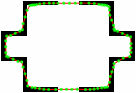
\includegraphics[width=\textwidth]{firstgvf}
		\caption{GVF snake with default settings}
	\end{subfigure}
	\caption{Different results for matching snakes to the room.}
	\label{fig:ex2}
\end{figure}

\section*{Exercise 3}
Using a GVF snake with the settings $\alpha=0.2, \beta=2, \gamma=1, \kappa=0.9, D_\text{min}=0.5, D_\text{max}=3.5$ gives the results shown in \autoref{fig:ex3} after 100 iterations. The results are not perfect, but this is about as well as I could make it. Changing $D_\text{max}$ to 3 or 4 will slightly alter the results, making the snake smoother but also changing the distance from the edge of the lungs in some places. It moves both closer to the edge and further away depending on the position.

\begin{figure}
	\centering
	\begin{subfigure}[t]{.45\textwidth}
		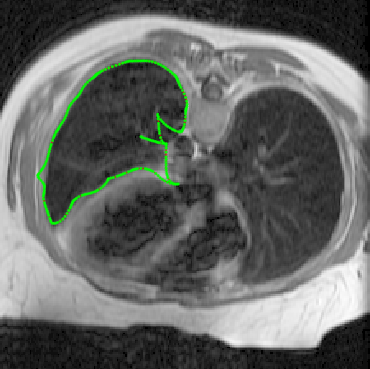
\includegraphics[width=\textwidth]{leftgvf}
		\caption{Left lung}
	\end{subfigure}~
	\begin{subfigure}[t]{.45\textwidth}
		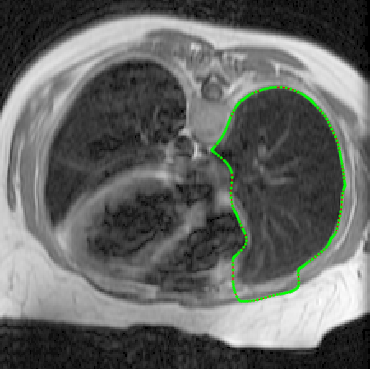
\includegraphics[width=\textwidth]{rightgvf}
		\caption{Right lung}
	\end{subfigure}
	\caption{Matching the lungs using the GVF snake using the settings $\alpha=0.2, \beta=2, \gamma=1, \kappa=0.9, D_\text{min}=0.5, D_\text{max}=3.5$.}
	\label{fig:ex3}
\end{figure}

\section*{Exercise 4}
The GVF snake on the high contrast image is shown in \autoref{fig:ex4}, the same settings were used. It seems that the results are worse than the for the left lung in \autoref{fig:ex3}. However the initial position is worse for the high contrast image so that will influence the result, this is especially visible on the top right where the initial position is quite far from the actual shape while for \autoref{fig:ex3} it is closer to the correct shape. The bottom left has about an equal initial position and there we can see that there is not a very large difference.

\begin{figure}
	\centering
	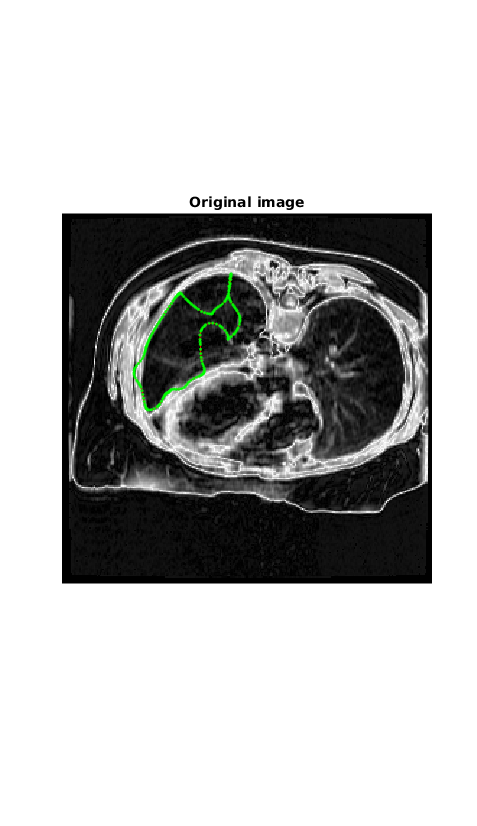
\includegraphics[width=.75\textwidth]{ex4}
	\caption{Using the high contrast and a GVF snake image to identify the left lung.}
	\label{fig:ex4}
\end{figure}
\section*{Exercise 5}
\section*{Exercise 6}

\end{document}